\documentclass[lettersize,journal]{IEEEtran}

% IEEE Transactions / Journals authoring format (IEEEtran V1.8b).
% Do not invent received/revised/accepted dates or volume/issue headers.

\usepackage{cite}
\usepackage{amsmath,amssymb,amsfonts}
\usepackage{array}
\usepackage[caption=false,font=normalsize,labelfont=sf,textfont=sf]{subfig}
\usepackage{textcomp}
\usepackage{url}
\usepackage{graphicx}
\usepackage[T1]{fontenc}
\usepackage[utf8]{inputenc}
\usepackage{xcolor}
\usepackage{booktabs}
\usepackage{multirow}
\usepackage{balance}
\usepackage[hidelinks]{hyperref}

\begin{document}
\bstctlcite{IEEEtran:BSTcontrol}

\title{Graph-Based and Self-Supervised Knowledge Tracing in Sparse-Concept Settings: A Critical Survey}

\author{Anonymous Authors
\thanks{Manuscript submitted to IEEE Transactions on Learning Technologies.
Author names, affiliations, emails, and ORCIDs are omitted for this anonymous copy.}
}

\markboth{IEEE Transactions on Learning Technologies}%
{Anonymous: Graph/SSL Knowledge Tracing in Sparse-Concept Settings}

\maketitle

\begin{abstract}
Knowledge Tracing (KT) is the sequential student-modeling engine of Intelligent Tutoring Systems (ITS), adaptive platforms, and Educational Data Mining (EDM): it estimates mastery over Knowledge Components (KCs) from interaction logs. Graph-Based KT (Graph-KT) and Self-Supervised KT (SSL-KT) have expanded rapidly as responses to isolated ID embeddings and long-tail concepts, yet evaluation under sparse-concept, cold-start, and calibration conditions is not standardized. This paper is a PRISMA 2020-informed systematic survey of 37 primary-core studies (2018--2026) identified from six bibliographic databases plus arXiv preprint monitoring ($N = 2,017$). We classify Graph-KT by codebook provenance and encoder family, and SSL-KT by locked pretext family, yielding $N_G = 36$, $N_S = 9$, and $N_{G \cap S} = 8$. Coding shows that none of the 37 studies isolate a strict zero-exposure KC split and that none of the 37 manuscripts report Expected Calibration Error (ECE). Those gaps are learning-technology constraints for new-KC onboarding, log-derived skill maps, and mastery actions from raw $P(r=1)$. As a survey-computed \texttt{REPRODUCED} overlay---not a change to the $0/37$ manuscript-reporting claim---we also report equal-width ECE on author DyGKT/ASSIST17 (one model, one dataset, one seed). Relative to prior TLT-scoped KT maps, the deliverable is a critical audit plus an operational GO/NO-GO checklist for those three tutoring decisions, with design recommendations for trustworthy and deployment-aware KT. The agenda puts corpus-derived priorities (zero-exposure benchmarks, calibration reporting, train-only graphs) before open technical directions.
\end{abstract}

\begin{IEEEkeywords}
Knowledge Tracing, Educational Data Mining, Graph Neural Networks, Self-Supervised Learning, Intelligent Tutoring Systems.
\end{IEEEkeywords}

% ─────────────────────────────────────────────────────────────────────────────
% SECTION 1: INTRODUCTION
% ─────────────────────────────────────────────────────────────────────────────
\section{Introduction}
\label{sec:intro}

\IEEEPARstart{K}{nowledge} Tracing (KT) is the fundamental task of sequentially modeling student mastery over educational Knowledge Components (KCs, e.g., concepts, skills, rules) based on historical learning interaction logs. In modern Intelligent Tutoring Systems (ITS), Educational Data Mining (EDM), and adaptive learning environments, Knowledge Tracing serves as the algorithmic engine for personalized learning pathways, learner-state estimation, step-based scaffolding, and automated curriculum adaptation. Formally, given a sequence of $T$ student interaction tuples $\mathcal{X}_{1:T} = \{(x_1, r_1), (x_2, r_2), \dots, (x_T, r_T)\}$, where $x_t \in \mathcal{E}$ represents the exercise or concept attempted at time $t$, and $r_t \in \{0, 1\}$ indicates the binary response accuracy (0 for incorrect, 1 for correct), the goal of Knowledge Tracing is to predict the response probability $P(r_{T+1} = 1 \mid x_{T+1}, \mathcal{X}_{1:T})$ on a target exercise $x_{T+1}$. Table~\ref{tab:notation_summary} summarizes the principal mathematical notations used throughout this survey.

\begin{table*}[t]
\caption{Summary of Key Mathematical Notations}
\label{tab:notation_summary}
\centering
\footnotesize
\begin{tabular}{@{}lp{0.78\textwidth}@{}}
\toprule
\textbf{Symbol} & \textbf{Mathematical Definition / Meaning} \\
\midrule
$\mathcal{X}_{1:T}$ & Sequential interaction history of a student up to time $T$ \\
$x_t, r_t$ & Exercise/concept attempted at time $t$ and binary response $r_t \in \{0,1\}$ \\
$\mathcal{E}, \mathcal{K}$ & Repository sets of exercises and Knowledge Components (KCs) \\
$\mathbf{A} \in \mathbb{R}^{|\mathcal{K}| \times |\mathcal{K}|}$ & Concept graph adjacency matrix (co-occurrence / prerequisite) \\
$h_k^t \in \mathbb{R}^d$ & Dynamic hidden knowledge state representation of concept $k$ \\
$\mathbf{Z}^{(v)}$ & Node/view representation embedding matrix from GNN view $v$ \\
$\tau$ & Temperature hyperparameter in InfoNCE contrastive loss \\
$W$ & Treatment/exposure in the open causal-debiasing agenda (not adjacency $\mathbf{A}$ and not history $\mathcal{X}_{1:T}$) \\
$\text{ECE}$ & Expected Calibration Error (equal-width bins; manuscript-reporting audit $0/37$; one REPRODUCED overlay in Sec.~\ref{sec:reliability}) \\
\bottomrule
\end{tabular}
\end{table*}

Since the seminal Deep Knowledge Tracing (DKT) model \cite{Piech_DKT_2015} introduced Recurrent Neural Networks (RNNs) to sequence modeling in education, deep sequence models---including Attention-based KT (SAKT \cite{Pandey_SAKT_2019}, AKT \cite{Ghosh_AKT_2020}) and Memory Network KT (DKVMN \cite{Zhang_DKVMN_2017})---have become the standard predictive baselines over classic psychometric models such as Bayesian Knowledge Tracing (BKT) and Item Response Theory (IRT).

\subsection{Learning-Technology Motivation: Data Sparsity \& Cold-Start}
Despite recent empirical progress, traditional deep KT architectures treat exercise and concept identifiers as independent categorical tokens, ignoring explicit domain structures and educational relationships. This formulation faces two recurring challenges in real-world intelligent tutoring systems:
\begin{enumerate}
    \item \textbf{Sparse-interaction representations}: In realistic educational platforms, interaction matrices are extremely sparse. Most students attempt only a tiny fraction of the overall item repository, and long-tail concepts receive minimal interaction logs. Sequence models that treat IDs as isolated tokens therefore have little evidence from which to estimate embeddings for those concepts---a motivation widely stated in the Graph-KT and SSL-KT literature, not a collapse statistic measured in this survey.
    \item \textbf{Strict Concept Cold-Start}: When new concepts or exercises are introduced into a curriculum without prior historical interaction logs, conventional deep KT models cannot infer student mastery from interaction IDs alone. Handling zero-exposure concepts during curriculum adaptation requires incorporating external structural, pedagogical, or semantic knowledge graph priors.
\end{enumerate}

\subsection{Scope \& Gateway Criteria}
To address these fundamental limitations, two primary methodological paradigms have rapidly expanded:
\begin{itemize}
    \item \textbf{Graph-Based Knowledge Tracing (Graph-KT)}: Incorporating explicit graph or graph-structured relations (e.g., concept prerequisite trees, question-KC bipartite maps, or dynamic co-occurrence graphs) as a central structural mechanism, including but not limited to Graph Neural Network (GNN) message passing. A Graph-KT paper need not use a GNN.
    \item \textbf{Self-Supervised Knowledge Tracing (SSL-KT)}: Formulating an auxiliary pretext objective on sequences or graphs (e.g., multi-view contrast, bipartite graph reconstruction, or sequence contrast) to regularize student-state representations. Exclusive family codes are the locked codebook tokens; PEBG is \texttt{GRAPH\_RECONSTRUCTION}, not a masked auto-encoder.
\end{itemize}

Our systematic survey enforces a strict, frozen primary-corpus gateway rule:
\begin{equation}
\begin{split}
\text{PRIMARY\_CORE} = \; & \text{KT} \land (\text{GRAPH\_BASED} \\
& \lor \text{SELF\_SUPERVISED})
\end{split}
\end{equation}

Only studies where Knowledge Tracing is the central prediction task AND that leverage explicit Graph-Based or Self-Supervised mechanisms are included in our primary synthesis corpus.

\subsection{Comparison with Prior Reviews and Benchmarks}
Prior reviews cover broad KT \cite{Abdelrahman_Survey_2023}, TLT-scoped KT models, variants, and applications \cite{Shen_KTSurvey_2024}, deep-KT tooling and empirical comparison under standard splits \cite{Liu_pyKT_2022,Liu_DLKT_2025}, and Graph-KT structure/propagation \cite{Xu_GbKT_2026}. Those works are complementary, not incorrect. This paper does not claim to be the first KT or Graph-KT review. It is a narrower operational audit: Graph-KT and SSL-KT only, coded for graph provenance, SSL pretext family, strict KC versus item versus learner cold-start, ECE reporting, and tutoring-deployment implications. Table~\ref{tab:survey_comparison} records those differences of scope.

For TLT readers, Shen \textit{et al.} remain the broad learning-technology map of KT. The present paper does not replace that survey. A reader who already knows Shen still needs this paper for three jobs Shen does not code: (i)~whether a published Graph/SSL-KT protocol supports \emph{new-KC} onboarding versus only interaction sparsity, (ii)~whether a log-derived graph may be treated as a pedagogical skill map, and (iii)~whether raw $P(r=1)$ may trigger remediation without a calibration report. Those jobs are answered with locked sparse/cold-start fields, provenance$\times$encoder coding, an ECE manuscript-reporting audit ($0/37$) plus one \texttt{REPRODUCED} overlay, and the GO/NO-GO checklist in Sec.~\ref{sec:go_nogo}.

\begin{table*}[t]
\caption{Comparison with Prior Knowledge Tracing Reviews and Benchmark Suites}
\label{tab:survey_comparison}
\centering
\footnotesize
\setlength{\tabcolsep}{3.4pt}
\begin{tabular}{@{}>{\raggedright\arraybackslash}p{2.15cm}
>{\raggedright\arraybackslash}p{2.25cm}
>{\raggedright\arraybackslash}p{2.35cm}
>{\raggedright\arraybackslash}p{2.25cm}
>{\raggedright\arraybackslash}p{2.35cm}
>{\raggedright\arraybackslash}p{2.55cm}@{}}
\toprule
\textbf{Dimension} & \cite{Abdelrahman_Survey_2023} & \cite{Liu_pyKT_2022,Liu_DLKT_2025} & \cite{Shen_KTSurvey_2024} & \cite{Xu_GbKT_2026} & \textbf{This survey} \\
\midrule
Protocol & Narrative / semi-systematic & Empirical tool + review & Narrative TLT review & Graph-KT survey (JEDM) & PRISMA 2020-informed; $N=2{,}017$ \\
Graph-KT & High-level GNN overview & Sequence-first; GKT as one DLKT model & Graph-KT as one DL variant & Structure $\times$ propagation & Provenance $\times$ encoder ($N_G=36$) \\
SSL-KT & Minimal / none & Not an SSL-KT taxonomy & Not a dedicated SSL-KT taxonomy & Not an SSL-KT survey & Four locked S-criterion families ($N_S=9$) \\
Sparse / cold-start & Generic sparsity & Standard interaction splits & Learning-process variants & Dataset catalogue, not a zero-exposure ontology & Interaction sparsity vs item / learner / strict KC \\
Provenance / split & Not audited & Benchmark splits for DLKT & Not audited & Not a leakage/provenance audit & Split/provenance coded; no locked leakage \% \\
ECE / trust & Not evaluated & AUC / ACC emphasis & Not evaluated & Not an ECE audit & Manuscript ECE $0/37$; one \texttt{REPRODUCED} overlay \\
Learning-technology use & Broad KT applications & Shared experimental protocol & Models, variants, applications & Graph structure for EDM & T1--T3 GO/NO-GO for ITS / adaptive / formative use \\
Artifacts & Citation index & pyKT repository & EduData / EduKTM & Dataset guidance & QA6 author-artifact coding; supplementary labels \\
\bottomrule
\end{tabular}
\end{table*}

\subsection{Main Contributions}
The contributions are framed for TLT readers (ITS, EDM, learning analytics, and trustworthy adaptive systems):
\begin{enumerate}
    \item \textbf{PRISMA-informed corpus and coding protocol}: Six core bibliographic databases plus arXiv preprint monitoring yield 2,017 records and a 37-paper primary core ($N_G=36$, $N_S=9$, $N_{G \cap S}=8$). Paper-, model-, and experiment-level labels are released as supplementary artifacts.
    \item \textbf{Two-dimensional taxonomy}: Graph-KT is classified by provenance (model-defined, external, or dynamically learned) and encoder family; SSL-KT is classified by the four locked codebook pretext families among $N_S=9$ papers.
    \item \textbf{Sparse-concept validity audit}: The coding separates generic interaction sparsity from item, learner, and strict KC cold-start. None of the 37 studies isolate a zero-exposure KC split. Item cold-start is YES for SINKT only ($1/37$).
    \item \textbf{Calibration and deployment-readiness audit}: None of the 37 manuscripts report ECE ($0/37$). One survey-computed \texttt{REPRODUCED} ECE overlay (DyGKT/ASSIST17; one model, one dataset, one seed) shows calibration can be measured from author artifacts; it does not establish corpus-wide calibration. Coded gaps remain tutoring-design constraints, not a reproduced accuracy ranking.
    \item \textbf{Design recommendations}: Section~\ref{sec:go_nogo} states a three-decision GO/NO-GO checklist for learning engineers; Section~\ref{sec:design_recs} states the five reporting rules those verdicts require. Corpus-derived agenda items precede open technical directions.
\end{enumerate}

This article is a Survey and Tutorial synthesis. It does not claim classroom outcomes, tutor-log A/B tests, or an executed \emph{pyKT-ColdStart} run; the learning-technology deliverable is the coded stop/go checklist above.

% ─────────────────────────────────────────────────────────────────────────────
% SECTION 2: SYSTEMATIC REVIEW METHODOLOGY
% ─────────────────────────────────────────────────────────────────────────────
\section{Systematic Review Methodology and PRISMA Protocol}
\label{sec:methodology}

This paper is a PRISMA 2020-informed systematic survey: identification, screening, eligibility, and inclusion are reported in the PRISMA 2020 flow structure (Fig.~\ref{fig:prisma_flow}) and are guided by the locked protocol. We report a locator-assisted coding-sample $\kappa$ and a separate independent-blind 20-paper $\kappa$ (Sec.~\ref{sec:icr}); we do not claim a completed screening or full-text reliability package. Count-based conclusions are protocol-coded audit findings rather than independently replicated meta-analytic estimates.

We address six core research questions:
\begin{itemize}
    \item \textbf{RQ1}: How are graphs constructed, represented, and validated in Graph-KT, and what is their data leakage risk?
    \item \textbf{RQ2}: What GNN architectures, temporal backbones, and fusion mechanisms are utilized in Graph-KT?
    \item \textbf{RQ3}: What self-supervised learning pretext tasks, augmentation strategies, and structure preservation mechanisms exist in SSL-KT?
    \item \textbf{RQ4}: How are sparse-concept and cold-start settings defined, operationalized, and evaluated?
    \item \textbf{RQ5}: What is the status of reproducibility, statistical rigor, calibration, and computational reporting in Graph/SSL-KT?
    \item \textbf{RQ6}: What research agenda follows from the coded gaps, and which items remain open inferences?
\end{itemize}

\subsection{Literature Search Architecture \& Database Executions}
We executed four search query families (\texttt{Q-G} Graph-KT, \texttt{Q-S} Self-Supervised KT, \texttt{Q-P} Sparse-Concept Lens, \texttt{Q-R} Reliability Lens) across the six core bibliographic databases locked in the protocol, covering 2015-01-01 to 2026-07-31, and used arXiv only for preprint monitoring:
\begin{enumerate}
    \item \textbf{Scopus} ($n = 531$ records)
    \item \textbf{Web of Science Core Collection} ($n = 344$ records)
    \item \textbf{ScienceDirect} ($n = 257$ records)
    \item \textbf{SpringerLink} ($n = 255$ records)
    \item \textbf{IEEE Xplore} ($n = 232$ records)
    \item \textbf{ACM Digital Library} ($n = 200$ records)
\end{enumerate}
arXiv contributed $n = 198$ additional preprint records. These six core runs plus preprint monitoring sum to $N = 2,017$ identified records.

\subsection{PRISMA 2020 Screening \& Eligibility Flow}
The systematic screening pipeline proceeded in four transparent stages (Fig.~\ref{fig:prisma_flow}):
\begin{enumerate}
    \item \textbf{Identification}: 2,017 total raw records retrieved across all database search runs.
    \item \textbf{Deduplication}: 1,267 duplicate records removed via automated 4-tier matching, yielding 750 unique deduplicated records.
    \item \textbf{Stage 1 Screening (Title/Abstract)}: 610 records excluded for failing basic relevance; 140 articles passed to full-text assessment.
    \item \textbf{Stage 2 Screening (Full-Text Eligibility)}: 103 articles excluded (98 with primary exclusion codes EC1--EC7, plus 5 additional records removed during corpus verification; record-level issues and final exclusion reasons are reported as Supplementary Table~S-PRISMA-5 in the file \texttt{supplementary/Table\_S-PRISMA-5.csv}), so $140 - 103 = 37$.
    \item \textbf{Final Primary Core Corpus}: \textbf{37 PRIMARY\_CORE papers}. The legacy seed list of 34 core records was used only for recall checking and is not a second inclusion total.
\end{enumerate}

\begin{figure}[!t]
\centering
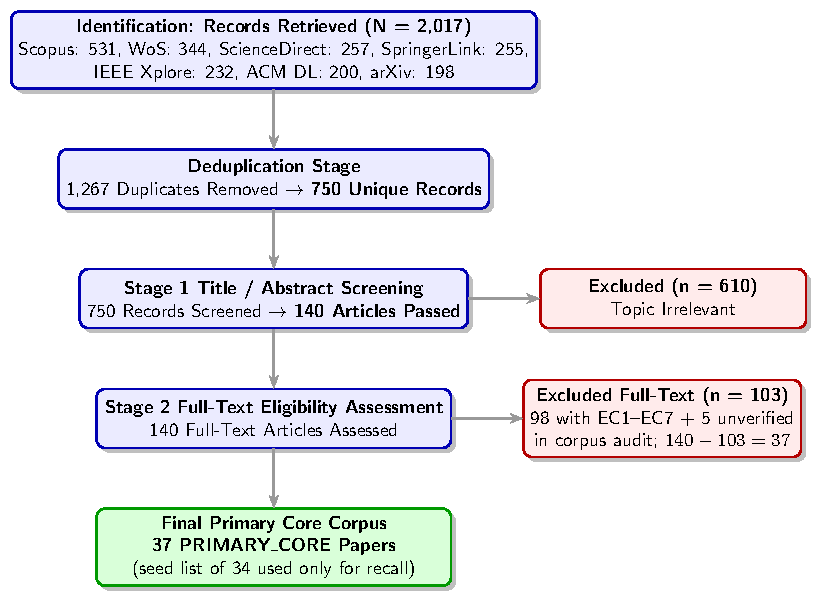
\includegraphics[width=\linewidth]{figures/fig_prisma_flow.pdf}
\caption{PRISMA 2020 reporting flow of search, deduplication, screening, and eligibility ($N = 37$ primary core papers; $N_{\text{raw}} = 2,017$ from six core databases plus arXiv preprint monitoring; $140 - 103 = 37$). Not a completed inter-rater reliability package.}
\label{fig:prisma_flow}
\end{figure}

\subsection{Evidence Coding Scheme}
To enforce methodological traceability, every study was coded across three linked levels: \textbf{PAPER}, \textbf{MODEL}, and \textbf{EXPERIMENT}. Field-level evidence tuples capture
\begin{equation}
\begin{aligned}
\text{Tuple} = \langle &\text{entity\_id},\; \text{field\_name},\; \text{coded\_value},\\
&\text{evidence\_locator},\; \text{evidence\_note} \rangle.
\end{aligned}
\end{equation}

\subsection{Quality \& Reliability Assessment Protocol}
We scored each study on codebook items QA1--QA8 ($0$--$2$). The total is a review-specific evidence-quality score for the present review, not a ranking of overall scientific quality. Normalized scores use $\mathrm{raw}/16$. Tiers are HIGH ($\ge 0.80$), MODERATE ($0.55$--$0.79$), and LIMITED ($< 0.55$).

QA7 scores how informative the evaluation design is for RQ4. It applies to all 37 primary-core papers because RQ4 asks how well each protocol supports sparse-concept inference, not because every author claimed to solve cold-start. The locked protocol (Sec.~22.1) permits QA7 to be coded \texttt{NA} when a paper makes no sparse or cold-start claim; this survey does not use that option, so the applicable maximum remains $16$.

Two review variables are kept separate from QA7. They are a coarse overlay from \texttt{sparse\_protocol\_category}, not a new abstract-level recode of all 37 papers. Claim values use locked ontology tokens. KT035 (HHSKT) is the documented exception: its protocol category remains \texttt{SPARSE\_INTERACTION\_ONLY}, but the paper reports an interaction-drop evaluation, so the overlay is not a generic 80/20 split. The 37-row file is \texttt{tables/H2\_qa7\_two\_variables.csv}.
\begin{center}
\footnotesize
\begin{tabular}{@{}rll@{}}
\toprule
$n$ & Evaluation regime & Sparsity claim \\
\midrule
35 & Generic split & No explicit focus \\
1 & Drop (HHSKT) & Generic data sparsity \\
1 & Item cold-start & Item cold-start \\
0 & Zero-exposure KC & Strict KC cold-start \\
\bottomrule
\end{tabular}
\end{center}
QA7 is applicable on every row of that overlay.

\subsection{Inter-Coder Reliability and Adjudication}
\label{sec:icr}
The locked protocol targets (i)~a 25\% second-screener sample of deduplicated title/abstract records plus all \texttt{UNCERTAIN} records, (ii)~second review of all \texttt{EXCLUDE\_FULLTEXT} / \texttt{UNCERTAIN} full-text decisions and at least 25\% of full-text eligibility decisions, and (iii)~double-coding of $\max(20, 25\%)$ primary-core papers (20 papers at $N=37$). Title/abstract and full-text pair files named in the protocol are not present; those stages were completed by a primary screener with team consensus on borderline cases. QA1--QA8 were assigned by the primary coder. The 20-paper coding sample (all nine S-criterion papers, all five H1 S=N papers, plus six Graph-only coverage rows) was double-coded on eight fields. Coder B (\texttt{NguyenKT}) used a quote locator pack, so this is not a fully independent blind pass. Pre-adjudication agreement was $158/160$ cells. For invariant fields on which both coders assigned the same category to all 20 papers (\texttt{strict\_kc\_cold\_start}, \texttt{learner\_cold\_start}, \texttt{ece\_reported}: all NO), percent agreement was $100\%$, whereas Cohen's $\kappa$ is undefined because the expected agreement $p_e=1$; those three fields were therefore excluded from the macro-average $\kappa$. On the five fields with defined $\kappa$, Coder A versus \texttt{NguyenKT} yields $1.00$ (S-criterion), $0.92$ (\texttt{ssl\_family}), $0.93$ (\texttt{graph\_provenance}), $1.00$ (\texttt{gnn\_encoder}), and $1.00$ (\texttt{item\_cold\_start}); the unweighted mean over those five defined values is $0.97$. Two cells were adjudicated to the locked gold (KT011 exclusive family $\texttt{MULTIVIEW\_CONTRASTIVE}$; KT026 provenance $\texttt{MODEL\_DEFINED\_FIXED}$). A second coder (\texttt{DaoMT}) independently double-coded the same 20-paper sample without a locator pack. Pre-adjudication agreement was $157/160$ cells; after excluding the same three invariant fields, the unweighted mean of the five defined field-wise $\kappa$ values is $0.96$ (S-criterion $1.00$; \texttt{ssl\_family} $0.92$; \texttt{graph\_provenance} $0.92$; \texttt{gnn\_encoder} $0.94$; \texttt{item\_cold\_start} $1.00$). Three cells were adjudicated to the locked gold (KT047 exclusive family $\texttt{MULTIVIEW\_CONTRASTIVE}$; KT070 provenance $\texttt{DYNAMIC\_LEARNED}$; KT068 encoder $\texttt{GNN\_GENERIC}$). The independent 20-paper $\kappa$ is not pooled with the locator-assisted coefficient. Pair tables and the recomputation sheet are in the supplementary reliability package. Count-based conclusions remain protocol-coded audit findings, not a pooled-effect meta-analysis.

\subsection{Methodological Evidence Synthesis Strategy}
Synthesizing evidence across Graph-KT, SSL-KT, and sparse evaluation protocols proceeded via qualitative thematic coding, structural taxonomy clustering, and count distributions of coded fields (not a pooled-effect meta-analysis).

% ─────────────────────────────────────────────────────────────────────────────
% SECTION 3: GRAPH-BASED KNOWLEDGE TRACING
% ─────────────────────────────────────────────────────────────────────────────
\section{Taxonomy and Synthesis of Graph-Based Knowledge Tracing (RQ1 \& RQ2)}
\label{sec:graph_kt}

Graph-Based Knowledge Tracing (Graph-KT) incorporates explicit graph topologies to model structural dependencies between Knowledge Components, questions, and student interaction histories. Paper-level coding of the 37-study corpus yields $N_G = 36$ Graph-KT papers (97.3\%); only CL4KT is sequence-only SSL. Fig.~\ref{fig:taxonomy_2d} presents the taxonomy axes used in this survey.

\begin{figure*}[t]
\centering
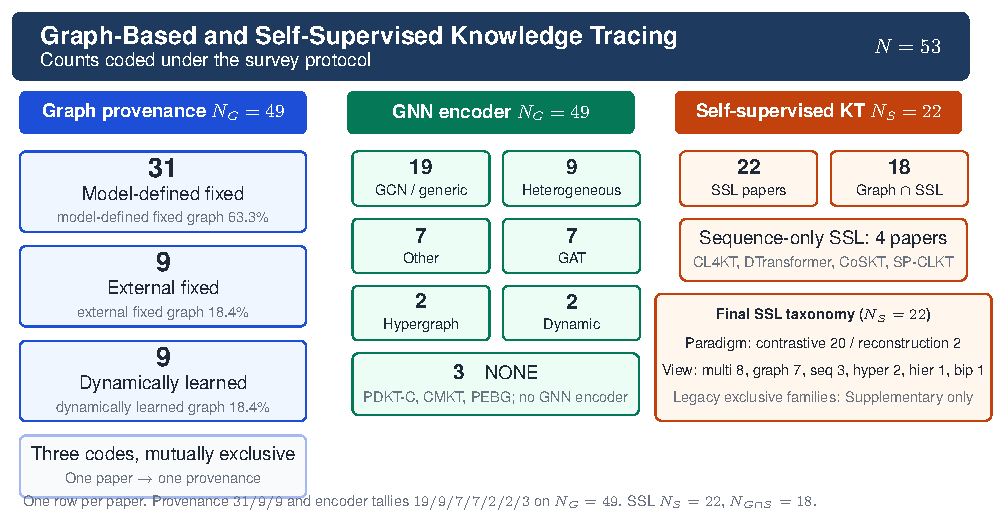
\includegraphics[width=0.78\linewidth]{figures/fig_taxonomy_2d.pdf}
\caption{Taxonomy axes coded under the locked survey protocol: $N=37$ papers; $N_G=36$ (CL4KT has \texttt{graph\_source=NONE}); provenance $18/9/9$; $N_S=9$; $N_{G\cap S}=8$.}
\label{fig:taxonomy_2d}
\end{figure*}

\subsection{Graph Provenance}
Paper-level coding of the 36 Graph-KT studies uses the protocol field \texttt{graph\_provenance} (Fig.~\ref{fig:graph_pipeline}). Counts are unique papers, not GKT Dense/Transition variants:
\begin{enumerate}
    \item \textbf{\texttt{MODEL\_DEFINED\_FIXED} ($n=18/36$, 50.0\%)}: The authors specify a fixed graph (Q-matrix, co-occurrence schema, session graph, and similar constructions) that is not learned as a free adjacency during training.
    \item \textbf{\texttt{EXTERNAL\_FIXED} ($n=9/36$, 25.0\%)}: The graph is supplied from an external source (expert prerequisite maps, concept maps, skill maps, or LLM/semantic graphs coded as external).
    \item \textbf{\texttt{DYNAMIC\_LEARNED} ($n=9/36$, 25.0\%)}: The adjacency or interaction graph is updated as part of training (including Coda's learnable code-graph \(A_u\)).
\end{enumerate}

\begin{figure*}[t]
\centering
\subfloat[Graph provenance: \texttt{MODEL\_DEFINED\_FIXED} $n=18$, \texttt{EXTERNAL\_FIXED} $n=9$, \texttt{DYNAMIC\_LEARNED} $n=9$ ($N_G=36$; mutually exclusive).]{%
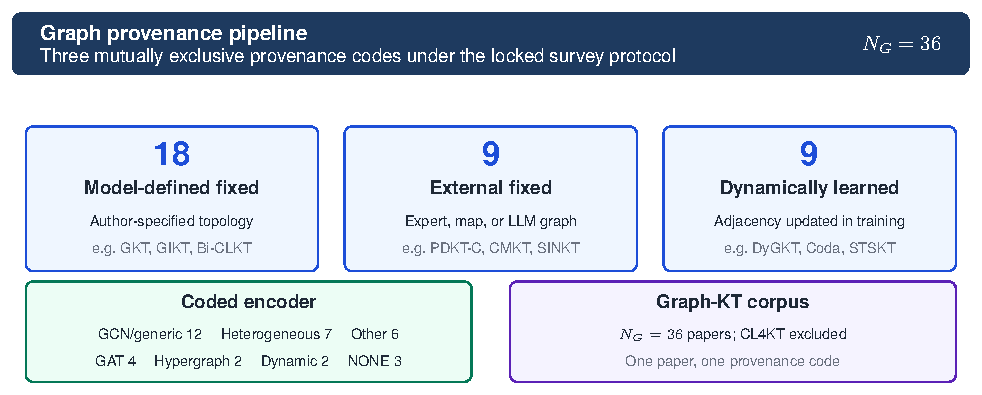
\includegraphics[width=0.48\textwidth,height=1.85in,keepaspectratio]{figures/fig_graph_construction_pipeline.pdf}%
\label{fig:graph_pipeline}}
\hfill
\subfloat[Encoder counts ($N_G=36$; mutually exclusive): GCN/generic $12$, \texttt{HETEROGENEOUS\_GNN} $7$, Other $6$, \texttt{GAT} $4$, hypergraph $2$, dynamic $2$, \texttt{NONE} $3$ (PDKT-C, CMKT, PEBG).]{%
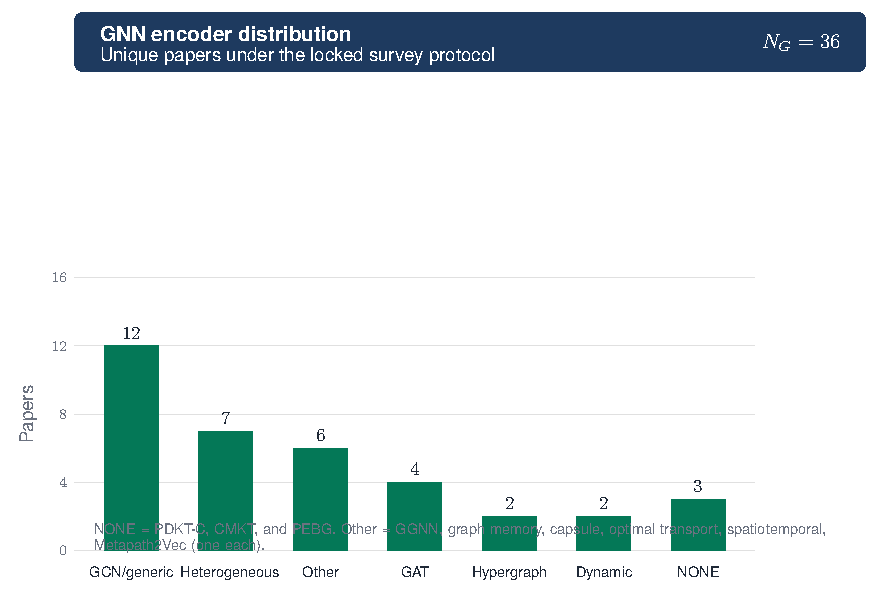
\includegraphics[width=0.48\textwidth,height=1.85in,keepaspectratio]{figures/fig_meta_analysis_charts.pdf}%
\label{fig:meta_charts}}
\caption{Locked graph-taxonomy counts: provenance (left) and encoder family (right).}
\label{fig:graph_counts}
\end{figure*}

\subsection{GNN Encoder Architectures}
Coded \texttt{gnn\_encoder} values on the 36 Graph-KT papers are shown in Fig.~\ref{fig:meta_charts}. Display grouping follows the CSV (one paper each; KT004 and HKT are \texttt{GNN\_GENERIC}):
\begin{itemize}
    \item \textbf{GCN / generic ($n=12/36$)}: \texttt{GCN} ($n=10$) plus \texttt{GNN\_GENERIC} ($n=2$; GKT, HKT). PEBG is not a GCN. A typical GCN update is:
    \begin{equation}
    \mathbf{H}^{(l+1)} = \sigma\left(\tilde{\mathbf{D}}^{-\frac{1}{2}} \tilde{\mathbf{A}} \tilde{\mathbf{D}}^{-\frac{1}{2}} \mathbf{H}^{(l)} \mathbf{W}^{(l)}\right)
    \end{equation}
    where $\tilde{\mathbf{A}} = \mathbf{A} + \mathbf{I}_{|\mathcal{K}|}$ adds self-loops and $\tilde{\mathbf{D}}$ is the corresponding degree matrix.
    \item \textbf{\texttt{HETEROGENEOUS\_GNN} ($n=7/36$)}.
    \item \textbf{\texttt{GAT} ($n=4/36$)}.
    \item \textbf{\texttt{HYPERGRAPH\_GNN} ($n=2/36$)} and \textbf{\texttt{DYNAMIC\_GNN} ($n=2/36$)}.
    \item \textbf{\texttt{NONE} ($n=3/36$)}: PDKT-C, CMKT, and PEBG use an explicit graph (or bipartite relation) without a GNN encoder. PEBG pretrains embeddings with a product-based neural network.
    \item \textbf{Other ($n=6/36$)}: \texttt{GGNN}, \texttt{GRAPH\_MEMORY}, \texttt{CAPSULE\_GNN}, \texttt{GRAPH\_OPTIMAL\_TRANS}, \texttt{SPATIOTEMPORAL\_GNN}, and KSG-AKT \texttt{OTHER} (Metapath2Vec + convolutional embedding; one paper each).
\end{itemize}

\subsection{Temporal Integration \& State Fusion Mechanisms}
To predict student performance sequentially, Graph-KT models combine structural embeddings with temporal backbones coded in the CSV (RNN/LSTM/GRU, self-attention, memory networks, or continuous Hawkes). Tables~\ref{tab:graph_taxonomy} and~\ref{tab:graph_taxonomy_b} list all 36 Graph-KT papers.

\begin{table*}[t]
\caption{Graph-KT coding under the locked survey protocol ($N_G=36$; one row per paper; 18 of 36). Display labels are readable forms of locked codebook values. PDKT-C, CMKT, and PEBG have no GNN encoder. GKT is counted as \texttt{MODEL\_DEFINED\_FIXED}; Dense versus Transition constructions are in the supplementary model-entry table.}
\label{tab:graph_taxonomy}
\centering
\footnotesize
\setlength{\tabcolsep}{3.5pt}
\begin{tabular}{@{}ll>{\raggedright\arraybackslash}p{2.15cm}l>{\raggedright\arraybackslash}p{1.55cm}lll@{}}
\toprule
\textbf{Paper} & \textbf{Model} & \textbf{Graph source} & \textbf{Provenance} & \textbf{Nodes} & \textbf{Encoder} & \textbf{Temporal} & \textbf{Fusion} \\
\midrule
\textbf{KT004} & GKT \cite{KT004_GKT_2019} & Multiple graph variants & Model-defined & KC--KC & Generic GNN & RNN & Concat \\
\textbf{KT010} & GIKT \cite{KT010_GIKT_2021} & Q-matrix & Model-defined & Exercise--KC & GAT & RNN & Attentive \\
\textbf{KT011} & Bi-CLKT \cite{KT011_BiCLKT_2022} & Co-occurrence & Model-defined & Dual subgraph & GCN & Attention & GNN state \\
\textbf{KT012} & JKT \cite{KT012_JKT_2021} & Q-matrix + co-occ. & Model-defined & Exercise--KC & GCN & RNN & Attentive \\
\textbf{KT014} & PDKT-C \cite{KT014_PDKTC_2018} & Expert prerequisite & External & KC--KC & none & RNN & Regularizer \\
\textbf{KT016} & SKT \cite{KT016_SKT_2020} & Co-occurrence & Model-defined & KC--KC & GAT & RNN & Attentive \\
\textbf{KT023} & SGKT \cite{KT023_SGKT_2022} & Session graph & Model-defined & Interaction & GGNN & RNN & Concat \\
\textbf{KT026} & Pretrain Q-Emb \cite{KT026_PretrainQ_2020} & Q-matrix & Model-defined & Exercise--KC & none / PNN pretrain & RNN & Embedding init \\
\textbf{KT029} & DGEKT \cite{KT029_DGEKT_2024} & Dynamic co-occ. & Dynamic & KC--KC & GCN & RNN & Attentive \\
\textbf{KT031} & KSG-AKT \cite{KT031_KSGAKT_2022} & Knowledge structure & External & KC--KC & Other & Attention & Attentive \\
\textbf{KT033} & DGMN \cite{KT033_DGMN_2023} & Dynamic interaction & Dynamic & Exercise--KC & Graph memory & Memory & GNN state \\
\textbf{KT035} & HHSKT \cite{KT035_HHSKT_2023} & Heterogeneous schema & Model-defined & Student--ex.--KC & Heterogeneous & RNN & Attentive \\
\textbf{KT036} & TSKT \cite{KT036_TSKT_2024} & Text semantics & External & Exercise--KC & Heterogeneous & RNN & Attentive \\
\textbf{KT037} & CMKT \cite{KT037_CMKT_2022} & Concept map & External & KC--KC & none & RNN & Regularizer \\
\textbf{KT038} & DyGKT \cite{KT038_DyGKT_2024} & Dynamic interaction & Dynamic & Interaction & Dynamic GNN & RNN & Attentive \\
\textbf{KT042} & S2-HHN \cite{KT042_S2HHN_2023} & Hypergraph schema & Model-defined & Student--ex.--KC & Hypergraph & RNN & Attentive \\
\textbf{KT043} & 3V-CLKT \cite{KT043_3VCLKT_2024} & Three-view graph & Model-defined & Student--ex.--KC & Heterogeneous & RNN & Attentive \\
\textbf{KT044} & SINKT \cite{KT044_SINKT_2024} & LLM semantic & External & KC--KC & GAT & Attention & Attentive \\
\bottomrule
\end{tabular}
\end{table*}

\begin{table*}[t]
\caption{Graph-KT coding under the locked survey protocol (remaining 18 of $N_G=36$).}
\label{tab:graph_taxonomy_b}
\centering
\footnotesize
\setlength{\tabcolsep}{3.5pt}
\begin{tabular}{@{}ll>{\raggedright\arraybackslash}p{2.15cm}l>{\raggedright\arraybackslash}p{1.55cm}lll@{}}
\toprule
\textbf{Paper} & \textbf{Model} & \textbf{Graph source} & \textbf{Provenance} & \textbf{Nodes} & \textbf{Encoder} & \textbf{Temporal} & \textbf{Fusion} \\
\midrule
\textbf{KT047} & DC-SSL \cite{KT047_DCSSL_2023} & Dual-channel & Model-defined & Exercise--KC & Heterogeneous & Attention & Attentive \\
\textbf{KT050} & GraphCA \cite{KT050_GraphCA_2023} & Context-aware & Model-defined & Exercise--KC & Heterogeneous & RNN & Attentive \\
\textbf{KT052} & Capsule GNN \cite{KT052_CapsuleGNN_2022} & Capsule graph & Model-defined & KC--KC & Capsule & RNN & Concat \\
\textbf{KT053} & GASKT \cite{KT053_GASKT_2021} & Q-matrix & Model-defined & Exercise--KC & GCN & Attention & Attentive \\
\textbf{KT056} & LST-Graph \cite{KT056_LSTGraph_2025} & Long-short graph & Dynamic & KC--KC & GAT & RNN & Attentive \\
\textbf{KT060} & STHKT \cite{KT060_STHKT_2025} & Spatiotemporal Hawkes & Dynamic & Interaction & GCN & Hawkes & GNN state \\
\textbf{KT062} & LGS-KT \cite{KT062_LGSKT_2025} & Logical-grammatical & External & KC--KC & GCN & RNN & Attentive \\
\textbf{KT063} & MAHKT \cite{KT063_MAHKT_2025} & Multi-association & Model-defined & Student--ex.--KC & Heterogeneous & RNN & Attentive \\
\textbf{KT064} & MG-Ensemble \cite{KT064_MGEnsemble_2025} & Multi-granularity & Model-defined & Exercise--KC & GCN & RNN & Attentive \\
\textbf{KT065} & CS-GKT \cite{KT065_CSGKT_2025} & Concept structure & Model-defined & KC--KC & GCN & RNN & Attentive \\
\textbf{KT066} & HyperKT \cite{KT066_HyperKT_2025} & Dual hypergraph & Model-defined & State hypergraph & Hypergraph & Attention & Attentive \\
\textbf{KT067} & SKM-GKT \cite{KT067_SKMGKT_2025} & Skill map & External & KC--KC & GCN & RNN & Concat \\
\textbf{KT068} & HKT \cite{KT068_HKT_2025} & Hierarchical & External & KC--KC & Generic GNN & Attention & Attentive \\
\textbf{KT069} & AEGOT-CDKT \cite{KT069_AEGOTCDKT_2025} & Optimal transport & Dynamic & KC--KC & Optimal transport & RNN & Attentive \\
\textbf{KT070} & Coda \cite{KT070_Coda_2025} & Covariate-debiased & Dynamic & KC--KC & GCN & RNN & Attentive \\
\textbf{KT076} & KGNN-KT \cite{KT076_KGNNKT_2025} & LLM knowledge graph & External & Exercise--KC & Heterogeneous & RNN & Attentive \\
\textbf{KT077} & R$^2$GCurL \cite{KT077_R2GCurL_2026} & Curriculum graph & Dynamic & Interaction & Dynamic GNN & RNN & Attentive \\
\textbf{KT079} & STSKT \cite{KT079_STGSKT_2026} & Streaming graph & Dynamic & Interaction & Spatiotemporal & RNN & Attentive \\
\bottomrule
\end{tabular}
\end{table*}

\subsection{Methodological Risk: Data Leakage in Log-Derived Graphs}
A methodological risk remains when a graph is built from interaction logs without a documented train-only construction rule. The locked survey protocol does not code a single leakage percentage, so we do not report one. Papers whose \texttt{graph\_source} is log-derived (for example \texttt{COOCCURRENCE\_SIMILARITY}, \texttt{SEQUENTIAL\_TRANSITION}, \texttt{DYNAMIC\_COOCCURRENCE}) require an explicit split statement before the adjacency can be treated as leakage-free. Learning-technology consequences for this risk are summarized in Table~\ref{tab:its_implications}.

% ─────────────────────────────────────────────────────────────────────────────
% SECTION 4: SELF-SUPERVISED KNOWLEDGE TRACING
% ─────────────────────────────────────────────────────────────────────────────
\section{Taxonomy and Synthesis of Self-Supervised Knowledge Tracing (RQ3)}
\label{sec:ssl_kt}

Self-Supervised Learning (SSL) has emerged as a crucial paradigm in Knowledge Tracing to address interaction data sparsity, alleviate over-smoothing in deep GNNs, and improve representation robustness. Within our primary core corpus of 37 studies, 9 papers satisfy the locked S-criterion (a self-generated pretext or consistency target). Five other Graph-KT papers (SINKT, Coda, KGNN-KT, R$^2$GCurL, STSKT) satisfy the G-criterion but not the S-criterion: they use inductive, denoising, LLM-graph, curriculum/RL, or streaming-graph mechanisms without a self-generated pretext or consistency target. Fig.~\ref{fig:ssl_framework} illustrates pretext-family axes used in this survey.

\begin{figure*}[t]
\centering
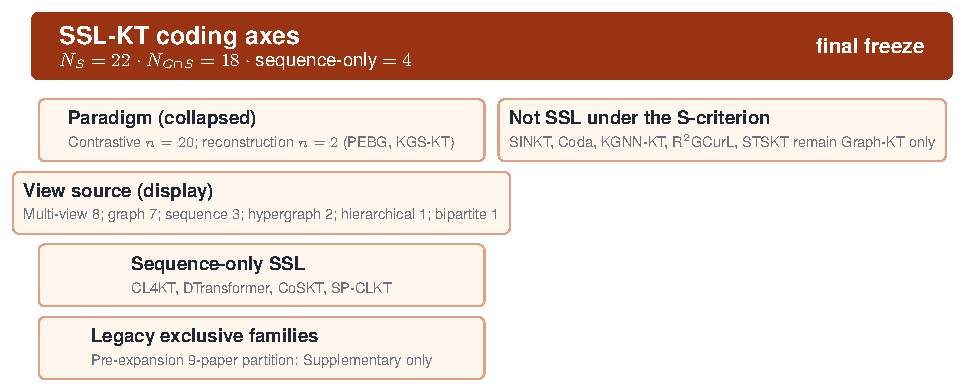
\includegraphics[width=0.92\linewidth]{figures/fig_ssl_framework.pdf}
\caption{SSL-KT families under locked codebook Sec.~14 tokens: $N_S=9$ papers and 4 exclusive \texttt{ssl\_family} codes. $N_{G\cap S}=8$; CL4KT is sequence-only.}
\label{fig:ssl_framework}
\end{figure*}

\subsection{SSL Objective Taxonomy}
The locked S-criterion codes 9 papers into four exclusive codebook families (Fig.~\ref{fig:ssl_framework}; Table~\ref{tab:ssl_taxonomy}). Hypergraph, line-graph, and hierarchical wording in the table are mechanism notes, not extra family codes:
\begin{enumerate}
    \item \textbf{Multiview contrast ($n=5$)}: Bi-CLKT, S2-HHN, 3V-CLKT, DC-SSL, HyperKT. A common contrastive objective is InfoNCE:
    \begin{equation}
    \mathcal{L}_{\text{InfoNCE}} = -\log \frac{\exp\left(\text{sim}(\mathbf{z}_i^{(1)}, \mathbf{z}_i^{(2)}) / \tau\right)}{\sum_{j=1}^B \exp\left(\text{sim}(\mathbf{z}_i^{(1)}, \mathbf{z}_j^{(2)}) / \tau\right)}
    \end{equation}
    where $\mathbf{z}_i^{(1)}, \mathbf{z}_i^{(2)}$ are normalized view embeddings, $\tau$ is temperature, and $B$ is batch size.
    \item \textbf{Graph contrast ($n=2$)}: GraphCA, HKT.
    \item \textbf{Graph reconstruction ($n=1$)}: PEBG / Pre-train Q-Emb (bipartite Q--S reconstruction, not masked concept prediction).
    \item \textbf{Sequence contrast ($n=1$)}: CL4KT.
\end{enumerate}

\subsection{Augmentation Strategies \& Perturbation Operators}
SSL-KT models employ stochastic augmentation operators over interaction sequences and graph structures:
\begin{itemize}
    \item \textbf{Sequence Perturbations}: Item masking, interaction cropping, random insertion, and timeline shuffling.
    \item \textbf{Graph Topology Perturbations}: Edge dropping, node attribute masking, sub-graph random walks, and counterfactual rewiring.
\end{itemize}

\subsection{Educational Structure Preservation}
Auxiliary SSL losses regularize student state representations. In contrastive models such as CL4KT \cite{KT039_CL4KT_2022}, sequence augmentations must satisfy \texttt{NO\_EXPLICIT\_CONSTRAINT} on structural validity, as random item masking creates hard negative views that force the model to learn invariant skill representations.

\subsection{Graph + SSL Intersection Paradigm}
Eight primary core papers ($N_{G \cap S} = 8$) combine an explicit graph mechanism with a self-supervised objective (all SSL-KT papers except sequence-only CL4KT). Table~\ref{tab:ssl_taxonomy} lists all 9 SSL-KT studies.

\begin{table*}[t]
\caption{SSL-KT coding under locked codebook Sec.~14 ($N_S=9$). Family is the exclusive locked token. Mechanism is a readable note, not a family code. Structure = whether an explicit educational graph is retained.}
\label{tab:ssl_taxonomy}
\centering
\footnotesize
\setlength{\tabcolsep}{3.0pt}
\begin{tabular}{@{}l>{\raggedright\arraybackslash}p{2.15cm}>{\raggedright\arraybackslash}p{1.85cm}>{\raggedright\arraybackslash}p{1.85cm}>{\raggedright\arraybackslash}p{2.05cm}l>{\raggedright\arraybackslash}p{1.45cm}@{}}
\toprule
\textbf{Paper} & \textbf{Model} & \textbf{SSL family} & \textbf{Mechanism} & \textbf{Augmentation} & \textbf{Train.} & \textbf{Structure} \\
\midrule
\textbf{KT011} & Bi-CLKT \cite{KT011_BiCLKT_2022} & Multiview contrast & Node + graph views & Edge dropout / subgraph & Joint & Graph retained \\
\textbf{KT026} & Pre-train Q-Emb (PEBG) \cite{KT026_PretrainQ_2020} & Graph reconstruction & Bipartite Q--S & Relation reconstruction & Two-st. & Graph retained \\
\textbf{KT039} & CL4KT \cite{KT039_CL4KT_2022} & Sequence contrast & Subsequence views & Crop / reorder / mask & Joint & No graph constraint \\
\textbf{KT042} & S2-HHN \cite{KT042_S2HHN_2023} & Multiview contrast & Hypergraph views & Hyperedge masking & Joint & Graph retained \\
\textbf{KT043} & 3V-CLKT \cite{KT043_3VCLKT_2024} & Multiview contrast & Three graph views & Three-view perturbation & Joint & Graph retained \\
\textbf{KT047} & DC-SSL \cite{KT047_DCSSL_2023} & Multiview contrast & Dual-channel views & Channel masking & Joint & Graph retained \\
\textbf{KT050} & GraphCA \cite{KT050_GraphCA_2023} & Graph contrast & Counterfactual views & Graph perturbation & Joint & Graph retained \\
\textbf{KT066} & HyperKT \cite{KT066_HyperKT_2025} & Multiview contrast & Hypergraph / line-graph & Dual-view masking & Joint & Graph retained \\
\textbf{KT068} & HKT \cite{KT068_HKT_2025} & Graph contrast & Hierarchical levels & Hierarchical perturbation & Joint & Graph retained \\
\bottomrule
\end{tabular}
\end{table*}

The 9 SSL-KT manuscripts \emph{report} that pretext objectives regularize representations under interaction sparsity. This survey does not reproduce a collapse-prevention or accuracy effect. Deployment implications are in Table~\ref{tab:its_implications}.

% ─────────────────────────────────────────────────────────────────────────────
% SECTION 5: SPARSE-CONCEPT & COLD-START EVALUATION
% ─────────────────────────────────────────────────────────────────────────────
\section{Sparse-Concept \& Cold-Start Evaluation Protocols (RQ4)}
\label{sec:sparse_coldstart}

A central contribution of our survey is clarifying the construct ambiguity surrounding "sparsity" in Knowledge Tracing literature. We distinguish between two fundamentally different evaluation settings (Table~\ref{tab:sparse_taxonomy}):
\begin{enumerate}
    \item \textbf{Generic Interaction Data Sparsity}: Student interaction logs are randomly partitioned (e.g., 80/20 train/test learner split). While the overall interaction matrix is sparse, \textbf{every Knowledge Component (KC) appears in the training split}. All 37 studies report generic interaction sparsity; none isolate a strict zero-exposure KC hold-out.
    \item \textbf{Strict Zero-Exposure KC Cold-Start}: A subset of KCs is completely withheld from training interaction logs (zero training exposure). No primary-core paper implements that split. SINKT \cite{KT044_SINKT_2024} evaluates a one-quarter \emph{question} hold-out and is coded YES for item cold-start, not for zero-exposure KC. HHSKT \cite{KT035_HHSKT_2023} evaluates interaction-drop sparsity and is coded \texttt{NO} for strict KC cold-start.
\end{enumerate}

\subsection{Methodological Audit of Evaluation Split Vulnerabilities}
Two construct risks recur in the literature; neither is reported here as a locked count:
\begin{itemize}
    \item \textbf{Train-only graph construction}: When a co-occurrence or item-similarity graph can be built from interaction logs, adjacency weights can leak test-set structure unless the paper documents a train-only construction rule. The locked protocol codes provenance and split transparency; it does not count how many papers used the full interaction matrix.
    \item \textbf{Inclusion criterion mismatch}: Models motivated by ``solving the cold-start problem'' often report standard AUC on random 80/20 splits in which every KC still appears in training.
\end{itemize}

\subsection{Methodological Analysis of Cold-Start vs. Generic Interaction Splits}
The following is a structural reading of model families, not a measured AUC or random-guess result on this corpus:
\begin{itemize}
    \item \textbf{Standard transductive sequence models (e.g., DKT, SAKT, AKT)}: Depend on fixed ID lookup embeddings. A withheld KC has no training embedding unless an external prior is supplied. This survey does not measure how close such models come to chance under that split.
    \item \textbf{Transductive Graph-KT models (e.g., GKT, GIKT, Bi-CLKT)}: Use GNN message passing over co-occurrence or prerequisite graphs. If the graph is precomputed over full logs or lacks out-of-vocabulary node features, held-out-KC behavior remains a structural question rather than a demonstrated inductive evaluation.
    \item \textbf{Inductive semantic-graph models (SINKT for item/question hold-out)}: SINKT \cite{KT044_SINKT_2024} uses LLM/semantic graph priors and is the only primary-core paper coded YES for item cold-start (one-quarter question hold-out). It is coded \texttt{NO} for a zero-exposure KC split. HHSKT \cite{KT035_HHSKT_2023} is coded \texttt{NO} for strict KC cold-start (interaction-drop sparsity only) and is not treated here as an inductive cold-start evaluation.
\end{itemize}

To standardize future evaluations, Section~\ref{sec:agenda} specifies a proposed benchmark suite (\emph{pyKT-ColdStart}). That suite is a research-agenda specification only; this paper does not report an executed run.

\begin{table*}[t]
\caption{Sparse/cold-start coding under the locked survey protocol ($N=37$). All 37 rows have generic data sparsity. Strict KC cold-start YES: $0/37$. Item cold-start YES: $1/37$ (SINKT question hold-out). Learner cold-start YES: $0/37$. Display labels: Strict KC $=\texttt{STRICT\_KC\_COLD\_START}$; Item CS $=\texttt{ITEM\_COLD\_START}$; Sparse only $=\texttt{SPARSE\_INTERACTION\_ONLY}$. Table shows SINKT plus representative sparse-only rows. PEBG and KGNN-KT are sparse-only: they do not implement an item hold-out.}
\label{tab:sparse_taxonomy}
\centering
\footnotesize
\setlength{\tabcolsep}{3.2pt}
\begin{tabular}{@{}ll l ccc p{3.55cm}@{}}
\toprule
\textbf{ID} & \textbf{Model} & \textbf{Protocol} & \textbf{KC} & \textbf{Item} & \textbf{Learn.} & \textbf{Note} \\
\midrule
\textbf{KT044} & SINKT \cite{KT044_SINKT_2024} & Item CS & \textbf{NO} & YES & NO & Only item cold-start YES (question hold-out) \\
\textbf{KT026} & Pretrain Q-Emb \cite{KT026_PretrainQ_2020} & Sparse only & \textbf{NO} & NO & NO & Question-level sparsity; not item hold-out \\
\textbf{KT076} & KGNN-KT \cite{KT076_KGNNKT_2025} & Sparse only & \textbf{NO} & NO & NO & 7:2:1 + difficulty bins; not item hold-out \\
\textbf{KT035} & HHSKT \cite{KT035_HHSKT_2023} & Sparse only & \textbf{NO} & NO & NO & Interaction-drop; not strict KC \\
\textbf{KT004} & GKT \cite{KT004_GKT_2019} & Sparse only & \textbf{NO} & NO & NO & Generic sparsity only \\
\textbf{KT010} & GIKT \cite{KT010_GIKT_2021} & Sparse only & \textbf{NO} & NO & NO & Generic sparsity only \\
\textbf{KT011} & Bi-CLKT \cite{KT011_BiCLKT_2022} & Sparse only & \textbf{NO} & NO & NO & Generic sparsity only \\
\textbf{KT012} & JKT \cite{KT012_JKT_2021} & Sparse only & \textbf{NO} & NO & NO & Generic sparsity only \\
\textbf{KT038} & DyGKT \cite{KT038_DyGKT_2024} & Sparse only & \textbf{NO} & NO & NO & Generic sparsity only \\
\textbf{KT039} & CL4KT \cite{KT039_CL4KT_2022} & Sparse only & \textbf{NO} & NO & NO & Sequence SSL; \texttt{graph\_source=NONE} \\
\textbf{KT066} & HyperKT \cite{KT066_HyperKT_2025} & Sparse only & \textbf{NO} & NO & NO & Generic sparsity only \\
\textbf{KT068} & HKT \cite{KT068_HKT_2025} & Sparse only & \textbf{NO} & NO & NO & Generic sparsity only \\
\textbf{KT077} & R$^2$GCurL \cite{KT077_R2GCurL_2026} & Sparse only & \textbf{NO} & NO & NO & Generic sparsity only \\
\bottomrule
\end{tabular}
\end{table*}

Generic data sparsity is YES for all 37 papers. Strict KC cold-start is YES for $0/37$ papers. Item cold-start is YES for SINKT only ($1/37$). Learner cold-start is YES for $0/37$ papers. This survey does not report a reproduced cold-start AUC. See Table~\ref{tab:its_implications}.

% ─────────────────────────────────────────────────────────────────────────────
% SECTION 6: RELIABILITY, REPRODUCIBILITY & CALIBRATION AUDIT
% ─────────────────────────────────────────────────────────────────────────────
\section{Reliability, Reproducibility \& Calibration Audit (RQ5)}
\label{sec:reliability}

We scored the 37 primary core studies on codebook items QA1--QA8 (each $0$--$2$): QA1 task clarity; QA2 data/preprocessing transparency; QA3 split/provenance/leakage transparency; QA4 baseline/ablation adequacy; QA5 statistical uncertainty; QA6 author artifacts; QA7 sparse/cold-start construct validity; QA8 computational transparency. These items form an evidence-quality score for the present review, not a ranking of overall scientific quality. QA7 remains the RQ4 evidence-adequacy item (Sec.~\ref{sec:methodology}); scores are unchanged. Each paper is normalized by $16$. QA6 is capped at $2$. Extra inventory IDs KT078 and KT080--KT083 are excluded.

Using codebook thresholds on those QA6-capped sums, 11 studies meet the HIGH evidence-quality threshold of this review ($\ge 0.80$) and 26 meet MODERATE ($0.55$--$0.79$; mean $0.76$). No study falls in the LIMITED evidence-quality tier ($< 0.55$). The identifiers at the HIGH threshold are KT029, KT033, KT035, KT038, KT044, KT050, KT060, KT064, KT066, KT070, and KT077. That list is a reporting-adequacy partition for this review, not a ranking of scientific contribution.

\subsection{Computational Reporting (QA8)}
We did not extract wall-clock time, GPU memory, or paper-specific complexity formulas from the 37 manuscripts. Standard textbook GCN/GAT costs scale with edges, nodes, and embedding dimension, but those expressions are orientation only and are not coded results. QA8 records whether a paper reports computational transparency; implications for deployment cost are therefore limited to that reporting gap.

\subsection{Probability Calibration Audit (Expected Calibration Error)}
None of the 37 primary-core manuscripts report Expected Calibration Error (ECE). That locked manuscript-reporting count remains $0/37$ and is not a cross-paper calibration league table. This survey does not treat a specific confidence such as $P(r=1)>0.90$ as a corpus statistic. The agenda uses the standard equal-width definition across $M=10$ bins,
\begin{equation}
\text{ECE} = \sum_{m=1}^{M} \frac{|B_m|}{N} \left| \text{acc}(B_m) - \text{conf}(B_m) \right|,
\end{equation}
where $B_m$ is the set of predictions in $((m-1)/M, m/M]$.

As a single survey-computed \texttt{REPRODUCED} overlay---not a manuscript-reported corpus fact---we ran the author DyGKT implementation \cite{KT038_DyGKT_2024} on ASSIST17 (seed~$0$, author train/val/test ratios, transductive test edges, $n=94{,}156$) and obtained equal-width ECE~$=0.0361$ and Brier~$=0.1770$ (author-metric test AUC~$=0.8025$). That overlay is one model, one dataset, and one seed; it is not a benchmark ranking. It shows calibration \emph{can} be measured when author artifacts are available; it does not change the $0/37$ manuscript-reporting claim, does not establish calibration for the corpus as a whole, and does not license corpus-wide tutoring actions from raw $P(r=1)$. Implications for tutoring decisions remain in Table~\ref{tab:its_implications}; the supplementary package records the reproduction manifest, run log, and per-bin table.

% ─────────────────────────────────────────────────────────────────────────────
% SECTION 7: DISCUSSION
% ─────────────────────────────────────────────────────────────────────────────
\section{Discussion}
\label{sec:discussion}

\subsection{Synthesis of Graph-KT Contributions}
Our synthesis of the 36 Graph-KT studies shows that authors introduce explicit relational topologies---prerequisite maps, question--KC bipartite graphs, or dynamic interaction graphs---as a structural alternative to isolated categorical tokens. Cross-paper AUC gains versus DKT/SAKT are not treated as a league table.

\subsection{Synthesis of SSL-KT Contributions}
Authors of the 9 SSL-KT papers report that pretext objectives regularize student-state representations under interaction sparsity. That claim is synthesized from the source manuscripts; this survey does not reproduce a collapse-prevention effect. Eight papers combine an explicit graph mechanism with a self-supervised objective ($N_{G \cap S} = 8$).

\subsection{Architectural Mechanisms under Sparse \& Unseen Concept Conditions}
Zero-exposure KC evaluation is absent from the corpus ($0/37$). This survey therefore does \emph{not} report a reproduced degradation for GKT, CL4KT, or other models under that split. CL4KT has \texttt{graph\_source=NONE}, so a co-occurrence-edge explanation does not apply to it. A structural observation remains: ID-lookup transductive models have no training embedding for a withheld KC unless an external prior is supplied. That observation is not a measured AUC result.

\subsection{Learning-Technology Implications for Intelligent Tutoring Systems}
Table~\ref{tab:its_implications} translates coded gaps into learning-technology decisions for ITS, adaptive platforms, EDM, and formative assessment. Corpus basis is coded evidence under the locked survey protocol, not a reproduced benchmark and not a classroom result.

\begin{table*}[t]
\caption{Learning-technology decision table for ITS and adaptive platforms. Corpus basis is coded evidence under the locked survey protocol, not a reproduced benchmark and not a cross-paper league table.}
\label{tab:its_implications}
\centering
\footnotesize
\setlength{\tabcolsep}{2.8pt}
\begin{tabular}{@{}>{\raggedright\arraybackslash}p{0.17\textwidth}
>{\raggedright\arraybackslash}p{0.17\textwidth}
>{\raggedright\arraybackslash}p{0.20\textwidth}
>{\raggedright\arraybackslash}p{0.20\textwidth}
>{\raggedright\arraybackslash}p{0.18\textwidth}@{}}
\toprule
\textbf{Learning-technology decision} & \textbf{Evaluation risk} & \textbf{Required reporting before deployment} & \textbf{Corpus evidence} & \textbf{Practical implication} \\
\midrule
New KC or module onboarding.
\textit{TLT: ITS; adaptive systems} & Standard 80/20 AUC treats every KC as seen in training & Zero-exposure KC split plus an external or semantic prior & Strict KC cold-start YES: $0/37$. Item cold-start YES: SINKT only ($1/37$). HHSKT is interaction-drop, not that split. & Do not onboard a new module from a learner-level 80/20 split. \\
Log-derived graph construction.
\textit{TLT: EDM} & Test-set structure can enter adjacency weights & Train-only construction rule; do not claim a pedagogical prerequisite map without that statement & Split/provenance coded; no locked leakage rate. Log-derived \texttt{graph\_source} values need an explicit split statement. & Do not treat a log graph as a skill map until the split is documented. \\
Short learner histories.
\textit{TLT: adaptive systems; learning analytics} & Sparse logs are not the same as withheld KCs & Report the sparsity construct (interaction vs item vs learner vs KC) and the pretext target & $N_S=9$ papers \emph{report} SSL pretext regularizers; not reproduced here. & SSL is a reported regularizer, not demonstrated collapse prevention or calibrated mastery. \\
Using $P(r=1)$ for remediation or skipping.
\textit{TLT: formative assessment} & The calibration status of raw $P(r=1)$ is unverified in this corpus because none of the 37 manuscripts reports ECE & ECE and Brier (or equivalent) on the decision split & $0/37$ manuscripts report ECE. No corpus rate such as $P(r=1)>0.90$. & Calibration-unknown probabilities may be unsafe to use directly for tutoring decisions without calibration evidence. \\
Interpretable skill maps for scaffolding.
\textit{TLT: ITS; EDM ontologies} & Message passing is not the same as a readable prerequisite & Document graph source (expert/concept map vs log-derived) & \texttt{EXTERNAL\_FIXED} $n=9/36$; \texttt{gnn\_encoder=NONE} for PDKT-C and CMKT. & Graph-KT for interpretability does not require a GNN. \\
Calibration-aware ITS decision support.
\textit{TLT: trustworthy adaptive systems} & Acting on logits as mastery states & Pair predictive metrics with a decision rule (scaffold / review / adapt) and a calibration report & ECE reporting $0/37$; no locked classroom deployment. Temperature scaling is a recommendation, not a measured corpus result. & Predictive AUC is not a license to trigger curriculum actions. \\
\bottomrule
\end{tabular}
\end{table*}

\subsection{Three Tutoring Decisions: a GO/NO-GO Checklist}
\label{sec:go_nogo}
The checklist is an agenda inference from locked coding: it is not a classroom study, not a reproduced benchmark, and not a license to deploy. Apply the three decisions in order (new content, then graph interpretation, then probability actions).

\textbf{T1 --- Onboard a new KC or module.}
Coded evidence: strict KC cold-start YES is $0/37$. SINKT \cite{KT044_SINKT_2024} is coded YES only for item cold-start (one-quarter question hold-out), not zero-exposure KC. PEBG / Pre-train Q-Emb \cite{KT026_PretrainQ_2020} and KGNN-KT \cite{KT076_KGNNKT_2025} are coded \texttt{NO} for item cold-start. HHSKT is an interaction-drop protocol, not that split.
Verdict: \textbf{NO-GO} for new-KC onboarding from a learner-level 80/20 AUC. A new \emph{item} whose KCs already appear in training has only one coded YES protocol (SINKT). Required evidence before GO: a zero-exposure KC split plus an external or semantic prior (agenda A1).

\textbf{T2 --- Treat a graph as a scaffolding skill map.}
If the graph is an expert or concept map and no GNN is required for interpretability, two coded examples exist: PDKT-C \cite{KT014_PDKTC_2018} and CMKT \cite{KT037_CMKT_2022} (\texttt{EXTERNAL\_FIXED}, $\texttt{gnn\_encoder=NONE}$). If the graph is log-derived, this survey does not lock a leakage rate.
Verdict: \textbf{conditional GO} only when the source is a documented external map. \textbf{NO-GO} for calling a co-occurrence or transition graph a pedagogical prerequisite unless a train-only construction statement is reported.

\textbf{T3 --- Skip practice or assign remediation from $P(r=1)$.}
Coded evidence: manuscript-reported ECE is $0/37$; no corpus rate such as $P(r=1)>0.90$. The calibration status of raw $P(r=1)$ is therefore unverified in this corpus. The DyGKT/ASSIST17 \texttt{REPRODUCED} ECE overlay in Sec.~\ref{sec:reliability} demonstrates a measurable calibration number on one author codebase (single model/dataset/seed); it does not establish calibration for the corpus as a whole, is not a tutoring decision rule, and does not flip this corpus verdict.
Verdict: \textbf{NO-GO}. Required evidence before GO: ECE or Brier on the same split used for the tutoring action, plus an explicit rule for when a probability may trigger scaffold, review, or adapt. Temperature scaling is a recommended reporting practice, not a measured corpus result.

These three verdicts are why Table~\ref{tab:its_implications} is a deployment-constraint table, not an accuracy ranking.

\subsection{Design Recommendations for Trustworthy Graph/SSL Knowledge Tracing Systems}
\label{sec:design_recs}
The following recommendations are the reporting rules that would change a T1--T3 verdict from NO-GO to GO. They are critical readings of the locked coding, not classroom outcomes and not reproduced AUC or ECE values.

\textit{Recommendation 1 --- Strict KC cold-start (closes T1).} Do not claim concept cold-start support unless the evaluation uses a strict zero-exposure KC split. A standard learner-level 80/20 protocol leaves every KC visible in training and cannot license onboarding of a new module.

\textit{Recommendation 2 --- Train-only graphs (closes T2).} For log-derived graphs, report whether construction is train-only. Otherwise, deployment claims that treat the adjacency as a pedagogical skill map remain vulnerable to structural leakage. This survey does not lock a leakage percentage.

\textit{Recommendation 3 --- Calibration before action (closes T3).} Report calibration metrics such as ECE and Brier score when KT probabilities are used for mastery decisions, remediation, or skipping practice. Treat raw $P(r=1)$ as calibration-unknown until ECE, Brier score, or equivalent calibration evidence is reported ($0/37$ manuscripts report ECE).

\textit{Recommendation 4 --- Separate sparsity constructs (prevents T1/T2/T3 conflation).} Distinguish interaction sparsity, item cold-start, learner cold-start, and KC cold-start in both terminology and evaluation design. Generic data sparsity is YES for all 37 papers and is not evidence of any cold-start construct.

\textit{Recommendation 5 --- Pair prediction with a tutoring rule (operationalizes T3).} For ITS deployment, pair predictive metrics with an explicit learning-technology decision rule---when a predicted probability may trigger scaffolding, review, or curriculum adaptation---and state the evidence that rule requires. Predictive AUC alone is not that license.

\subsection{Methodological Limitations of the Present Survey}
Screening and coding were performed by the research team rather than by an independent external coder (Sec.~\ref{sec:icr}). This review synthesizes published protocols; \emph{pyKT-ColdStart} is a proposed evaluation specification only and is not an executed benchmark. The corpus spans papers through July 2026; LLM-KT work after the search cutoff falls outside the synthesis.

% ─────────────────────────────────────────────────────────────────────────────
% SECTION 8: RESEARCH AGENDA
% ─────────────────────────────────────────────────────────────────────────────
\section{Research Agenda (RQ6)}
\label{sec:agenda}

We separate two groups. Group~A follows coded gaps and should be closed before Graph-KT or SSL-KT is treated as deployment-ready. Group~B contains forward-looking technical directions; each is linked to a learning-technology need but is \emph{not} a coded result of the 37-paper audit. Group~A is the priority.

\subsection{Group A: Corpus-Derived Priorities}

\subsubsection{A1. Standardized Zero-Exposure KC Cold-Start Benchmarks (\emph{pyKT-ColdStart})}
This gap is coded: $37/37$ papers do not isolate a strict zero-exposure KC split. A held-out concept subset $\mathcal{K}_{\text{cold}} \subset \mathcal{K}$ is defined such that the training interaction count $n_{\text{train}}(k) = 0$ for every $k \in \mathcal{K}_{\text{cold}}$. The cold training interaction set $\mathcal{D}_{\text{train}}^{\text{cold}}$ is constructed via interaction-level filtering:
\begin{equation}
\mathcal{D}_{\text{train}}^{\text{cold}} = \{(x_t, r_t) \in \mathcal{D}_{\text{train}} \mid \text{KC}(x_t) \in \mathcal{K} \setminus \mathcal{K}_{\mathrm{cold}}\}
\end{equation}
where $\text{KC}(x_t)$ maps exercise $x_t$ to its constituent KCs. Models must infer response accuracy over $\mathcal{K}_{\text{cold}}$ at test time using external structural graphs or semantic priors. \emph{pyKT-ColdStart} is a specification only; this paper does not report an executed run.

\subsubsection{A2. Calibration and Trustworthy Probability Reporting}
This gap is coded: $0/37$ manuscripts report ECE, so the calibration status of raw $P(r=1)$ is unverified in this corpus. The DyGKT/ASSIST17 overlay in Sec.~\ref{sec:reliability} is survey-computed (\texttt{REPRODUCED}) on a single model/dataset/seed and does not close that manuscript-reporting gap or establish corpus-wide calibration. When tutoring systems use $P(r=1)$ to skip practice or assign remediation, raw logits $z_i$ should be converted to calibrated probabilities $\hat{p}_i = \sigma(z_i/T)$, with temperature $T>0$ fitted on a held-out validation set by minimizing negative log-likelihood, after which ECE and Brier score are evaluated on the test set. Temperature scaling remains a recommended reporting practice for future KT papers.

\subsubsection{A3. Train-Only Graph Construction and Leakage Reporting}
Log-derived \texttt{graph\_source} values (for example co-occurrence or sequential transition) require an explicit train-only construction statement before the adjacency is used as a skill map. The locked protocol codes provenance and split transparency; it does not lock a leakage percentage, and we do not invent one.

\subsubsection{A4. Reproducible Evidence Packages}
Future Graph/SSL-KT papers---and updates of this survey---should release split statements, graph-construction scripts or rules, calibration tables, and (for systematic reviews) pair-level inter-coder files. Screening and full-text second-screener pair files remain the open reliability task for the present protocol.

\subsection{Group B: Forward-Looking Technical Directions}

\subsubsection{B1. LLM-GNN Semantic Graph Fusion}
SINKT and KGNN-KT already use LLM or semantic graphs as \texttt{EXTERNAL\_FIXED} structure, but this survey does not measure a fusion architecture. For tutoring platforms that introduce new KCs by text (syllabus, textbook, or item stem), aligning LLM text representations $\mathbf{E}_{\text{LLM}} \in \mathbb{R}^{|\mathcal{K}| \times d_{\text{text}}}$ with GNN states $\mathbf{H}_{\text{GNN}} \in \mathbb{R}^{|\mathcal{K}| \times d_{\text{graph}}}$ is a candidate inductive prior:
\begin{equation}
\begin{split}
\mathbf{Z}_{\text{aligned}} = \; & \text{Softmax}\left(\frac{(\mathbf{E}_{\text{LLM}}\mathbf{W}_Q)(\mathbf{H}_{\text{GNN}}\mathbf{W}_K)^T}{\sqrt{d}}\right) \\
& \times (\mathbf{H}_{\text{GNN}}\mathbf{W}_V)
\end{split}
\end{equation}
where $\mathbf{W}_Q, \mathbf{W}_K \in \mathbb{R}^{d_{\text{text}} \times d}$ and $\mathbf{W}_V \in \mathbb{R}^{d_{\text{graph}} \times d}$ are learnable projections. This remains an open implementation, not a coded result.

\subsubsection{B2. Hyperbolic Knowledge-State Manifolds}
This is an open direction, not a coded encoder in the 37-paper corpus. Prerequisite and concept-map ITS often assume hierarchy; a Poincaré distance on student concept states $u, v \in \mathbb{B}^d = \{x \in \mathbb{R}^d \mid \|x\| < 1\}$ is
\begin{equation}
d_{\mathbb{B}}(u, v) = \text{arcosh}\left(1 + 2 \frac{\|u - v\|^2}{(1 - \|u\|^2)(1 - \|v\|^2)}\right).
\end{equation}
The learning-technology motivation is compact representation of deep skill trees, not a claim that hyperbolic KT was observed in this corpus.

\subsubsection{B3. Continuous-Time Modeling via Neural ODEs}
This is not a coded Neural-ODE result. Adaptive platforms log irregular practice intervals; a continuous state $h(t)$ with
\begin{equation}
h(t_{n+1}) = h(t_n) + \int_{t_n}^{t_{n+1}} f_\theta(h(\tau), \tau)\, d\tau
\end{equation}
is a candidate for forgetting and spaced practice. It does not replace the coded need for zero-exposure splits and ECE.

\subsubsection{B4. Causal Debiasing of Tutoring Logs}
This is an open direction. Popular items and attempt frequency can confound estimated mastery. If $Z$ is a sufficient observed confounder set, $P(Y \mid do(W = w)) = \sum_{z} P(Y \mid W = w, Z = z) P(Z = z)$. Interaction history remains $\mathcal{X}_{1:T}$ and the adjacency remains $\mathbf{A}$. Causal identification is not a coded property of the 37 papers.

% ─────────────────────────────────────────────────────────────────────────────
% SECTION 9: THREATS TO VALIDITY
% ─────────────────────────────────────────────────────────────────────────────
\section{Threats to Validity}
\label{sec:validity}

\textbf{Search completeness.} Four query families were executed on six core bibliographic databases plus arXiv preprint monitoring. Grey literature (workshop papers, technical reports, theses) was excluded per protocol, so relevant work outside those indexes may be absent.

\textbf{Selection and coding reliability.} Decisions were made by a primary screener, with borderline cases resolved by team consensus; QA1--QA8 were assigned by the primary coder. Screening and full-text second-screener pair files are not in the repository. The 20-paper coding sample reports field-wise Cohen's $\kappa$ in Sec.~\ref{sec:icr}: after excluding three invariant all-NO fields for which $\kappa$ is undefined ($p_e=1$), the locator-assisted mean over five defined $\kappa$ values is $0.97$ ($158/160$ cells) and an independent pass by \texttt{DaoMT} (no locator) yields mean $0.96$ over the same five defined fields ($157/160$). Those coefficients are not pooled. We release the coding schema, pair table, recomputed-$\kappa$ sheet, QA scores, and sparse/cold-start fields as supplementary artifacts.

\textbf{Construct validity of sparse and cold-start coding.} Generic data sparsity, item cold-start, learner cold-start, and strict KC cold-start are separate locked fields. A paper that discusses ``sparsity'' in prose is not recoded as YES for a construct it does not evaluate. Residual ambiguity remains where authors use ``cold-start'' for new items or short histories.

\textbf{External validity across datasets and platforms.} Coded studies typically report public interaction logs (commonly ASSISTments, EdNet, Statics, or Junyi). We did not lock a per-paper dataset inventory in the count CSVs, so we do not claim that every paper uses that exact set. Findings may not transfer to high-stakes assessment, workplace learning, or non-English logs. As a Survey and Tutorial article, this paper does not report classroom deployment outcomes; those are out of article-type scope. The learning-technology claim is limited to coded protocol constraints and the GO/NO-GO checklist.

\textbf{Temporal validity.} The search window is 2015--2026 (cutoff 2026-07-31). LLM-augmented KT is changing faster than a typical survey cycle; later systems fall outside this synthesis.

\textbf{Count-based survey versus reproduced benchmark.} This paper audits published protocols. It does not execute \emph{pyKT-ColdStart} and does not support a cross-paper AUC/ECE league table. One \texttt{REPRODUCED} ECE overlay on DyGKT/ASSIST17 is reported in Sec.~\ref{sec:reliability}; it is not a corpus re-ranking. Heterogeneous splits and seeds make pooled accuracy invalid. All quantitative comparisons remain within-study unless a matched protocol is stated.

% ─────────────────────────────────────────────────────────────────────────────
% SECTION 10: CONCLUSION
% ─────────────────────────────────────────────────────────────────────────────
\section{Conclusion}
\label{sec:conclusion}

This paper is a PRISMA 2020-informed critical survey of Graph-Based and Self-Supervised Knowledge Tracing under sparse-concept settings. Across 37 primary-core studies (2018--2026) identified from six core bibliographic databases plus arXiv preprint monitoring ($N = 2,017$), the TLT-facing contributions are as follows.

\textbf{Contribution 1 --- Protocol.} A PRISMA-informed corpus and reproducible coding schema for Graph/SSL-KT ($N_G=36$, $N_S=9$, $N_{G \cap S}=8$), with paper-level labels in the supplementary package.

\textbf{Contribution 2 --- Taxonomy.} Graph-KT is classified by provenance (model-defined $18$, external $9$, dynamically learned $9$) and encoder family, including three papers that use an explicit graph without a GNN (PDKT-C, CMKT, PEBG). SSL-KT is classified by four locked pretext families.

\textbf{Contribution 3 --- Validity audit.} Generic interaction sparsity is separated from item, learner, and strict KC cold-start. None of the 37 studies isolate a zero-exposure KC split; item cold-start is YES for SINKT only.

\textbf{Contribution 4 --- Calibration audit.} None of the 37 manuscripts report ECE ($0/37$). A single \texttt{REPRODUCED} equal-width ECE overlay on DyGKT/ASSIST17 (Sec.~\ref{sec:reliability}) shows calibration can be measured from author artifacts on one model/dataset/seed; it does not establish corpus-wide calibration, and raw $P(r=1)$ remains calibration-unknown for tutoring decisions in this corpus.

\textbf{Contribution 5 --- Design recommendations.} A three-decision GO/NO-GO checklist (new KC, skill-map graph, $P(r=1)$ action) plus five reporting rules constrain trustworthy KT deployment in ITS and adaptive systems. Corpus-derived agenda items (zero-exposure benchmarks, calibration reporting, train-only graphs, evidence packages) precede open technical directions.

The intended use is to give a learning engineer a coded stop/go before Graph-KT or SSL-KT informs tutoring---onboarding a new KC, treating a log-derived graph as a skill map, or acting on $P(r=1)$. It is not a cross-paper model league table.

\section*{Acknowledgment}
The authors used the Cursor AI coding assistant for language polishing, \LaTeX\ formatting, consistency checking, and implementation of author-approved manuscript and artifact revisions. All inclusion decisions, coding judgments, evidence interpretations, statistical decisions, and scientific conclusions were made and verified by the authors. AI-assisted changes were reviewed against the source literature and locked review protocol, and the authors take full responsibility for the final content.

\bibliographystyle{IEEEtran}
\bibliography{references}

\end{document}
